\documentclass[twoside, open=right
]{scrreprt}

%\usepackage{lmodern}
\usepackage{fouriernc}
\usepackage[T1]{fontenc}


\input{Qcircuit}

\usepackage[english]{babel}
\usepackage[utf8]{inputenc}
\usepackage{amsmath, amssymb, amsxtra}
\usepackage{xspace, braket}
\usepackage{setspace}
\usepackage{tikz}
\usepackage[european resistor, european voltage, european current]{circuitikz}

\usepackage{hyperref}
\hypersetup{
    bookmarks=false,         % show bookmarks bar?
    %unicode=false,          % non-Latin characters in Acrobat’s bookmarks
    %pdftoolbar=true,        % show Acrobat’s toolbar?
    %pdfmenubar=true,        % show Acrobat’s menu?
    pdffitwindow=false,     % window fit to page when opened
    pdfstartview={FitH},    % fits the width of the page to the window
    pdftitle={Quantum logic gates based on Rydberg atoms},    % title
    pdfauthor={Zubair Iftikhar},     % author
    pdfsubject={Quantum Phyiscs},   % subject of the document
    %pdfcreator={Creator},   % creator of the document
    %pdfproducer={Producer}, % producer of the document
    pdfkeywords={Rydberg atom} {Quantum information} {Anthropic principle}
}


\usepackage{sistyle} %Units
\usepackage{cleveref}
\usepackage{cancel}
\usepackage{lipsum}
%\usepackage{slashbox}

\usepackage{graphicx}
\usepackage[justification=centering]{caption}
\usepackage{subcaption}
\usepackage{wrapfig}

\renewcommand*{\dictumauthorformat}[1]{#1}

\usepackage[nottoc, notlof, notlot]{tocbibind}

\newcommand{\defi}{\xspace\ensuremath{\overset{\text{\tiny def}}{=}}\xspace}

\newcommand{\g}{\ensuremath{\ket{0}}\xspace}
\newcommand{\e}{\ensuremath{\ket{1}}\xspace}

\newcommand{\ff}{\ensuremath{\ket{g}}\xspace}
\newcommand{\ee}{\ensuremath{\ket{e}}\xspace}
\newcommand{\rr}{\ensuremath{\ket{r}}\xspace}
\newcommand{\bg}{\ensuremath{\bra{g}}\xspace}
\newcommand{\be}{\ensuremath{\bra{e}}\xspace}
\newcommand{\br}{\ensuremath{\bra{r}}\xspace}


\newcommand{\mat}{\emph{Mathematica}\xspace}
\newcommand{\matC}[1]{\textsl{\texttt{#1}}}

\newcommand{\dd}{\ensuremath{\mathrm d}\xspace}

\newcommand{\om}{\omega}
\newcommand{\Om}{\Omega}
\newcommand{\ga}{\gamma}
\newcommand{\Ga}{\Gamma}
\newcommand{\de}{\delta}
\newcommand{\De}{\Delta}
\newcommand{\ka}{\kappa}
\newcommand{\la}{\lambda}
\newcommand{\eps}{\epsilon}
\newcommand{\hlf}{\frac{1}{2}}
\newcommand{\mc}[1]{\mathcal{#1}}
\newcommand{\pp}{\mathcal{P}}
\newcommand{\sig}{\hat{\sigma}}
\newcommand{\Sig}{\hat{\Sigma}}
\newcommand{\hrho}{\hat{\rho}}
\newcommand{\Th}{\Theta}



\addtokomafont{chapter}{\rmfamily}

\titlehead{
\begin{small}
\begin{spacing}{1.1}
  A. V. Rzhanov Institute of Semiconductor Physics\hfill \today \\
  Siberian branch of the Russian Academy of Science \\
  Prospekt Lavrentieva 13 \\
  630090 Novosibirsk\\
  RUSSIA
\end{spacing}
\end{small}
\vspace{3cm}
\Large \center{\textsc{Intership report}}}
\subject{M2 NanoSciences \textsl{NanoPhysique Track}}
\title{\rmfamily \scshape Quantum logic gates based on \\ Rydberg atoms \vspace{5cm} }
\author{
  \textit{Author}\,: \hspace{3cm} \hfill Zubair \textsc{Iftikhar} \\
  \textit{Supervisor}\,: \hfill Ilya \textsc{Beterov} \\
  \textit{Jury}\,: \hfill Jean-Jacques \textsc{Greffet} \\
  \textit{Jury}\,: \hfill Yvan \textsc{Sortais}
}
\date{}

\pdfmapfile{=/usr/share/texmf/fonts/map/public/fourier/dvips/fourier/fourier.map}

\begin{document}
\maketitle

\addchap{Acknowledgements}

\par I would like to thank all the members of the Quantum Optics team of Akadiemgorodok: Ilya Beterov, my supervisor for all the kind advices he gave me all along my internship; Denis, for the tasty discussions we used to had at lunch time but not only; Vassia, for his attempts to talk in English every time; Aliona, the PhD student of Ilya, for the tour of the city and for the happiness she brought when she was here.

\par I also would like to gratefully thank Leonid, Igor, Alina Bogomolova, Michèle Debrenne, Sita Baby and Alan Swan for their help and the opportunity they gave to me to make this wonderful internship.

\par Last but not the least, I do not forget all the people that helped me to \emph{survive} four months in the wild and terrific Siberia.

\tableofcontents

\addchap{Introduction}

\dictum[Franz Kafka]{There is a goal, but no way; what we call a way is hesitation.}
\bigskip

\par According to Alain Aspect, there has been recently a revolution in Physics: people are now able to manipulate individual atoms. That leads some researchers to make experiments where one can obviously observe spectacular non-classical behaviours like the wave-particle duality or entangled quantum states. That kind of Physics is usually considered as \emph{fundamental} by opposition to the \emph{applied} field. Nevertheless, as the Mathematics branch of the \emph{Number theory} it may be applied to cryptography. On the one hand, the entanglement property can be used to securely exchange encryption key\footnote{Some commercial quantum cryptography systems are already available, the only limitation is the geographic distance between the two users indeed it requires optical fiber to send the keys, but in practice these fibers have attenuation and the cryptography protocol forbid repeaters.}. On the other hand, the superposition principle might be used to make a quantum computer and break some cryptography protocols like the ones that are used today for secure payment on the Internet. 

\par The idea of using quantum mechanics to make calculation has been first proposed by Yuri I. Manin and Richard Feynman in the 80's. Actually there are several ways to achieve this, after a decade of progress the enthusiasm has slowly decreased and today very few physicists are really trying to reproduce the architecture of classical computer to build the so called \emph{Quantum computer}. At first people tried to do so, but they were faced to fundamental issues linked to the coherence time of their atoms and also to technical problems because of the high complexity of these experimental setups. This conclusion led them to find tricky solutions like quantum simulator or hybrid systems. Nevertheless, our team is focussing on neutral atoms.

\par To understand basically what a quantum computer is, one has just to replace the classical bits on which are made usual calculations by bits obeying to quantum mechanics and then called \emph{qubits}. In particular a qubit can be in superposition of states \g and \e, where at a given time a classical bit can only be in one individual state either 0 or 1. That is why a quantum computer using qubits intrinsically allows \emph{parallelism}, as it will be explained in the first chapter.

\par All around the world, many teams are working on a two-level system that can be considered as a qubit: using two polarisations of the light, the number of photon in a cavity, the excitation level of electrons, its spin, the superconducting charge, etc. All these systems have their strengths and weaknesses. Some researchers are now trying to build hybrid systems, for instance they make operation on superconducting qubit and then store it in a nitrogen-vacancy center. But for now, the record of the largest number of entangled atoms is 14, and it has been reached with trapped ions.

\par Rydberg atoms are neutral atoms with an electron in highly excited state --- about $n=90$. As they are neutral, they are hard to trap. One can easily trap ions because of their charge, but to manipulate neutral atoms, laser cooling and a vacuum chamber are mandatory. Here, at the A.V.Rzhanov Institute of Semiconductor Physics SB RAS, the \emph{quantum optics} team works on Rubidium atoms. They are trying to observe Rydberg blockade with an original setup including a channeltron electron multiplier used as electron counter. This phenomenon consists in the inhibition of excitation by a Rydberg atom due to dipole-dipole interaction. In other words: in a cold atoms gas, only one can be simultaneously in a Rydberg state. This blockade can be used to implement a important quantum logical gate, namely the Controlled-NOT.

\par During my stay here, I was involved both in theory and experimentation. About theory, based on a recent article \cite{Molmer}, I have made a program to simulate some experiments and try to study and to validate a theoretical proposal of my tutor \cite{Ilya}; that job is detailed in the second chapter of this report. The next one deals with my experimental work in respect to the automation and the renew of the experimental setup. The first chapter is the summary of a bibliographic study and some lectures given by Leonid V. Il'ichov. I have attended these lectures to give a feedback on the education here, in Novosibirsk State University which is, for two years, a partner institution of the Institut d'Optique Graduate School.


\chapter{Quantum computation}

\par Binary number system and the associated Boolean algebra are at the basis of the computations made inside classical computers. The idea of \emph{quantum} computation is to use a two-level quantum state to replace the usual classical LOW and HIGH levels. These states cross the so called \emph{gates} to make basic logic operations like NOT, AND, etc.

\par The first part of this chapter will be about the general ideas of quantum computation. It is based on the 3 lectures given by Leonid V. Il'ichov I have attended during my stay in Akademgorodok. He taught an introduction to this interesting field underlying my work at the laboratory. He has first explained why a quantum computer is much more powerful than a classical one. To go further we will also show how a quantum computer can run all the operations and algorithm a classical computer can. He finished his lectures by talking about the Grover's algorithm but we will discuss the Deutsch-Jozsa problem.

\par Then we will discuss the practical implementation of a quantum logic gate using Rydberg blockade and understand why neutral atoms are good candidates for quantum computation. 

\section{Quantum logic gates}

\begin{wraptable}{r}{0.35\textwidth}
  \vspace{-10pt}
  \centering
  \begin{tabular}{||c|c||c||}
    \hline
    $x$ & $y$ & $x \oplus y$\\
    \hline \hline
    0 & 0 & 0\\
    0 & 1 & 1\\
    1 & 0 & 1\\
    1 & 1 & 0\\
    \hline
  \end{tabular}
  \caption{\label{XOR-tab} XOR truth table}
  \vspace{-10pt}
\end{wraptable}

\par Let us consider the quotient ring $\mathbb{Z}/2\mathbb{Z}$ with the logical XOR operation $\oplus$. This operation is defined by its truth table in \Cref{XOR-tab}.

\par A bit is an element of this ring. Using $n$ bits in a register $\{ x_0, x_1, ..., x_{n-1} \}$, one can represent a number $X = x_{n-1} \times 2^{n-1} + ... + x_1 \times 2 + x_0 \times 1$ between $0$ and $2^n-1$. There are in total $\mathcal{N} \defi 2^n$ possible representations.

\subsection{Quantum parallelism}
\par In the \emph{quantum world}, one uses typical two-level quantum system as bit. For instance two polarisations of the light (horizontal/vertical or circular right/circular left) could be used as a two-level system, as well as two states of excitation of an atom (ground state/excited state). These bits obey to the laws of quantum mechanics, that is why one uses Dirac notation for them: \g and \e\footnote{The qubits are vectors of $\mathbb{C}^2$, the two dimension Hilbert space on the complex number with the usual hermitian product and canonical basis \{\g,$\ket{1}$\}. A qubit is a physical state, it is thus always normalised.}.

\par A quantum register represents a number by the following operation: $\ket{X} = \ket{x_{n-1}} \otimes ... \otimes \ket{x_1} \otimes \ket{x_0}$. Here, the $\otimes$ operator is a tensorial product: each qubit of the register acts independently\footnote{They cannot be summed, as well as one cannot sum apples and peaches. To understand this notation, one should consider $\ket{X}$ as a vector with the coordinates $(x_{n-1}; ... ; x_1; x_0)$.}. As a qubit is a quantum two-level system, its main property is that it can be in a superposition of states \g and \e, like $\ket{x_k} = \alpha_0 \g + \alpha_1 \e$. And by extension, the quantum register can be in superposition.

\begin{wrapfigure}{l}{0.35\textwidth}
  \vspace{-15pt}
  \begin{align*}
    \Qcircuit @C=1em @R=0.1em {
      \lstick{\ket{x_0}} & \multigate{4}{U_f} & \rstick{\ket{x_0}} \qw \\
      \lstick{\ket{x_1}} & \ghost{U_f} & \rstick{\ket{x_0}} \qw \\
      \lstick{...} & \ghost{U_f} & \rstick{...} \qw \\
      \lstick{\ket{x_{n-1}}} & \ghost{U_f} & \rstick{\ket{x_{n-1}}} \qw \\
      \lstick{\ket{y}} & \ghost{U_f} & \rstick{\ket{y \oplus f(X)}} \qw
    }
  \end{align*}
  \caption{\label{function-f} A reversible function $f$}
  \vspace{-15pt}
\end{wrapfigure}

\par As there are boolean functions in the classical world, there are some functions that acts on quantum registers. But the \emph{Landauer principle} claims that during computation, an erasing of information is equivalent to dissipation. To avoid dissipation --- and by this way allow a quantum computer --- a boolean function should copy the input register at its output\footnote{By the pigeonhole principle, to be bijective, an injective function on a finite ensemble should be surjective.}. A quantum boolean function can then be represented as in the \Cref{function-f}, where $y$ is used to invert the output $f(X)$.

\par Then the input is: $\ket{X} \otimes \ket{y}$ and the output is: $\ket{X} \otimes \ket{y \oplus f(X)}$. There is no loss of information, moreover this quantum computer is doing a unitary operation. Indeed, if the input wave functions $\ket{X^{(k)}}$ are orthogonal, then the output $\ket{X^{(k)}} \otimes \ket{y \oplus f(X^{(k)})}$ are also orthogonal.

\par The superiority of quantum computers on the classical ones will soon become obvious. If one creates a superposition of register: $\alpha_1 \ket{X^{(1)}}  + \alpha_2 \ket{X^{(2)}}$ and use it as an input for the previous function, the input will be: $( \alpha_1 \ket{X^{(1)}}  + \alpha_2 \ket{X^{(2)}} ) \otimes \ket{y}$ and the output will be $\alpha_1 \ket{X^{(1)}} \otimes \ket{y \oplus f(X^{(1)})} + \alpha_2 \ket{X^{(2)}} \otimes \ket{y \oplus f(X^{(2)})}$. It means that one has called \emph{two times} the function $f$ using only one launch of the computer. If one manage to create a superposition of $n$ registers, then it can call $n$ times the function $f$ at the same time, this is called quantum parallelism.

\subsection{Universal gates}

\begin{wraptable}{r}{0.35\textwidth}
  \vspace{-10pt}
  \centering
  \begin{tabular}{||c|c||c||}
    \hline
    $x$ & $y$ & $x\ \mathrm{NAND} \ y$\\
    \hline \hline
    0 & 0 & 1\\
    0 & 1 & 1\\
    1 & 0 & 1\\
    1 & 1 & 0\\
    \hline
  \end{tabular}
  \caption{\label{NAND-tab} NAND truth table}
  \vspace{-10pt}
\end{wraptable}

\par In classical computation, it has been shown that any boolean function can be written using only NAND (or NOR) logic gate. This gate is then considered as universal. The problem is that this gate is obviously not reversible. Indeed, as shown in \Cref{NAND-tab}, the output "1" has several inputs.
\par Quantum logic gates  have to be reversible to avoid dissipation an let the hope to be able one day to make an actual quantum computer. Then, in principle, one cannot implement a classical NAND gate on a quantum computer. However it exists a reversible gate called Toffoli gate, that is a universal gate for classical computation. It employs 3-bits instead of the 2-bits NAND. This gate can be made using in particular two important 2-bits quantum logic gates: the Hadamard and the CNOT gates.

\subsubsection{Hadamard gate}

The Hadamard gate is a very basic gate but it will be widely used in this section. It is represented by a H and its behaviour is described in the \Cref{Hadamard-gate}.

\begin{figure}[h]
  \begin{subfigure}[b]{0.3\textwidth}
  \[
      \Qcircuit @C=0.7em @R=0.1em {
        \lstick{\g} & \gate{H} & \rstick{\frac{1}{\sqrt{2}} (\g + \e)} \qw
      }
  \]
  \caption{Input: \g}
  \end{subfigure}
  ~
  \begin{subfigure}[b]{0.3\textwidth}
  \[
    \Qcircuit @C=0.7em @R=0.1em {
      \lstick{\e} & \gate{H} & \rstick{\frac{1}{\sqrt{2}} (\g - \e)} \qw
    }
  \]
  \caption{Input: \e}
  \end{subfigure}
  ~
  \begin{subfigure}[b]{0.3\textwidth}
  \[
    \Qcircuit @C=0.7em @R=0.1em {
       \lstick{\ket{x}} & \gate{H} & \rstick{\frac{1}{\sqrt{2}} ((-1)^x \ket{x} + \ket{\bar{x}})} \qw
    }
  \]
  \caption{General input}
  \end{subfigure}
  \caption{\label{Hadamard-gate} Hadamard gate behaviours, $\bar{x}$ means NOT $x$}
\end{figure}

\par One may have noticed that if the input \g and \e are orthogonal, the outputs are also orthogonal. The matrix of this gate in the basis $\{ \g, \e \}$ is the following:
\[H = \frac{1}{\sqrt{2}} \begin{bmatrix}
1 &  1 \\
1 & -1 \end{bmatrix} \]
is called the Hadamard matrix and it has given its name to the gate. It is unitary.

\par Let us now compute the action of $n$ Hadamard gates on the qubits of a register $X$ of $n$ bits.

\begin{align*}
H^{\otimes n} \ket{X} &\defi H \ket{x_{n-1}} \otimes ... \otimes H \ket{x_1} \otimes H \ket{x_0} \\
    &= \frac{1}{\sqrt{2^n}}  \left( (-1)^{x_{n-1}} \ket{x_{n-1}} + \ket{\bar{x}_{n-1}} \right) \otimes ... \otimes \left( (-1)^{x_0} \ket{x_0} + \ket{\bar{x}_0} \right) \\
    &= \frac{1}{\sqrt{2^n}}  \sum_{Y=0}^{\mathcal{N}-1} \alpha(X,Y) \ket{Y}
\end{align*}
\par The summation is done over all the possible registers $Y$, $\ket{Y}=\ket{y_{n-1}} \otimes ... \otimes \ket{y_k} \otimes ... \otimes \ket{y_0}$. Then one needs to find the coefficients $\alpha(X,Y) = \pm 1$. First allow us to consider some few cases by the \Cref{coeff-alpha}.

\begin{table}[h]
  \centering
  \begin{tabular}{||c||c|c||}
    \hline
     & $x_k=0$ & $x_k=1$\\
    \hline \hline
    $y_k=0$ & 1 & 1\\ \hline
    $y_k=1$ & 1 & -1\\
    \hline
  \end{tabular}
  \caption{\label{coeff-alpha} Contribution of the $k^{\mathrm{th}}$ term to $\alpha(X,Y)$}
\end{table}

\par This table is made by taking the wave function $\ket{y_k}$, and trying all the cases. If $y_k = 0$ then the contribution will be $1$ because of the definition of $H$ (the sign of the projection on \g of the output is always positive). If $y_k = 1$, there are two cases, if $x_k = 0$ then it is also positive and if $x_k = 1$ then it is negative. It means that the sign is negative only if both $\ket{y_k}$ and $\ket{x_k}$ are in state \e. Thus the sign is $(-1)^{x_k \cdot y_k}$ and \[ \alpha(X,Y) = (-1)^{X \cdot Y} \text{, where }  X \cdot Y \defi x_{n-1} \cdot y_{n-1} \oplus ... \oplus x_1 \cdot y_1 \oplus x_0 \cdot y_0 \]

\par Here, the usage of the $\oplus$ operation on bits rather than simple addition is not mandatory. Finally it comes

\begin{equation}
  H^{\otimes n} \ket{X} = \frac{1}{\sqrt{2^n}}  \sum_{Y=0}^{\mathcal{N}-1} (-1)^{X \cdot Y} \ket{Y} \label{Hadamard}
\end{equation}


\subsubsection{CNOT gate}

\begin{wrapfigure}{r}{0.35\textwidth}
  \vspace{-20pt}
  \begin{align*}
    \Qcircuit @C=1em @R=1em {
      \lstick{\ket{x}} & \ctrl{1} & \rstick{\ket{x}} \qw \\
      \lstick{\ket{y}} & \targ & \rstick{\ket{y \oplus x}} \qw
     }
  \end{align*}
  \caption{\label{CNOT-scheme} CNOT gate}
  \vspace{-10pt}
\end{wrapfigure}

\par CNOT stands for Controlled-Not. It is a 2-bits gate: the first bit is called \emph{control} and the second one \emph{target}. Its truth table is given by a simple copy of the target if the control bit is down and the inversion otherwise. Its scheme is given by the \Cref{CNOT-scheme} where the dot represents the control bit, and the encircled cross the target bit.

\subsubsection{Toffoli gate}

\begin{wrapfigure}{r}{0.35\textwidth}
  \vspace{-20pt}
  \begin{align*}
    \Qcircuit @C=1em @R=1em {
      \lstick{\ket{x}} & \ctrl{1} & \rstick{\ket{x}} \qw \\
      \lstick{\ket{y}} & \ctrl{1} & \rstick{\ket{y}} \qw \\
      \lstick{\ket{z}} & \targ & \rstick{\ket{z \oplus xy}} \qw
     }
  \end{align*}
  \caption{\label{CCNOT-scheme} Toffoli gate}
  \vspace{-10pt}
\end{wrapfigure}


\par The Toffoli gate is actually a Controled-CNOT gate. One needs at least 3~bits to make reversible universal gate for classical computation. Indeed there are only two reversible gates with 2~bits: the identity gate and the CNOT gate. The schema of \Cref{Toffoli-equ} shows a circuit equivalent to the Toffoli gate based on Hadamard gate $H$, CNOT and T gate (which is a $\pi/4$-gate that just multiply the input by $e^{\pi/4}$). Thus using only this set of gates, one can in principle make a quantum computer that is able to run any classical algorithm. Moreover, these 3~gates are also a set of universal quantum logic gates \cite{Saff-rev}.


\begin{figure}[h]
  \begin{align*}
    \Qcircuit @C=0.8em @R=1em {
      \lstick{\ket{x}} & \qw & \qw & \qw & \ctrl{2} & \qw & \qw & \qw & \ctrl{2} & \qw & \ctrl{1} & \qw & \ctrl{1} & \gate{T} & \qw & \rstick{\ket{x}} \qw \\
      \lstick{\ket{y}} & \qw & \ctrl{1} & \qw & \qw & \qw & \ctrl{1} & \qw & \qw & \gate{T^{\dagger}} & \targ & \gate{T^{\dagger}} & \targ & \gate{T} & \gate{T} & \rstick{\ket{y}} \qw \\
      \lstick{\ket{z}} & \gate{H} & \targ & \gate{T^{\dagger}} & \targ & \gate{T} & \targ & \gate{T^{\dagger}} & \targ & \gate{T} & \gate{H} & \qw & \qw & \qw & \qw & \rstick{\ket{z \oplus xy}} \qw
     }
  \end{align*}
  \caption{\label{Toffoli-equ}This circuit is equivalent to a Toffoli gate}
\end{figure}

\subsection{Deutsch-Jozsa problem}

\par The problem of Deutsch and Jozsa is interesting to see how a quantum computer can work faster than a classical one. Let us consider a function $f$ as previously, the problem consist in guess whether the function is balanced\footnote{A function is called balanced when it return $1$ for one half of the inputs and $0$ for the other half.} or constant.

\par Using classical computation, the fastest solution is to try inputs all their tricks. Then, in the worst case, after $\mc{N}/2 +1$ operations the solution is found. If the output changed at the last operation it means that $f$ was balanced and it was constant otherwise.

\par Surprisingly, a quantum algorithm can solve the problem in only one single operation! Let us take an input with all qubits initialised at \g and the additional qubit at \e. Let us also \emph{sandwich} the function with Hadamard gates as shown in \Cref{Deutsch-pb}.

\begin{figure}[h]
  \begin{align*}
   \Qcircuit @C=1.5em @R=1em {
    \lstick{\ket{0}} & /^n \qw \ar@{--}[]+<0.8em,1em>;[d]+<0.8em,-2em> & \gate{H^{\otimes n}} \ar@{--}[]+<2em,1em>;[d]+<2em,-2em>  & \multigate{1}{U_f} \ar@{--}[]+<2em,1em>;[d]+<2em,-2em>  & \gate{H^{\otimes n}} \ar@{--}[]+<2em,1em>;[d]+<2em,-2em>  & \meter & \\
    \lstick{\ket{1}} & \qw     & \gate{H}             & \ghost{U_f}        & \qw \\
    & I & II & III & IV & V &
   }
  \end{align*}
  \caption{\label{Deutsch-pb}Deutsch-Jozsa algorithm}
\end{figure}

\par Here follows an explanation on the algorithm step by step: 

\begin{description}
  \item[$I$] \hfill \\ At first, the input is: \[ \g \otimes \g \otimes ... \otimes \g \otimes \e = \g^{\otimes n} \otimes \e \]
  \item[$II$] \hfill \\ Then all these qubits cross Hadamard gates. The $H^{\otimes n}$ applied to $\g^{\otimes n}$ gives a balanced superposition of all the possible registers: $H^{\otimes n} \g^{\otimes n} = 1 / \sqrt{2^n} \sum_{x=0}^{2^n-1} \ket{x}$. Then after this step, one gets: \[ \frac{1}{\sqrt{2^{n+1}}}\sum_{x=0}^{2^n-1} \ket{x} \otimes (\g - \e) \]
  \item[$III$] \hfill \\ This register goes into the function, then it comes: \[ \frac{1}{\sqrt{2^{n+1}}}\sum_{x=0}^{2^n-1} \ket{x} \otimes (\ket{f(x)} - \ket{1\oplus f(x)} ) \]
After this step, the additional qubit is not important anymore, but its sign gives the sign of each contribution to the register superposition: if $f(x)=0$ it is positive and otherwise it is negative\footnote{According to the following convention: $1/\sqrt{2^{n+1}}\sum_{x=0}^{2^n-1} (-1)^{f(x)} \ket{x} \otimes (\g - \e)$. The sign is inverted if one consider $\e - \g$ as additional qubit. But anyway, global phase does not matter in quantum mechanics.}.
  \item[$IV$] \hfill \\ The \Cref{Hadamard} yields \[ \frac{1}{2^n}\sum_{x=0}^{2^n-1} (-1)^{f(x)} \sum_{y=0}^{2^n-1}(-1)^{x\cdot y} \ket{y} \]
Then one can switch the two sums (because they are finite): \[ \frac{1}{2^n}\sum_{y=0}^{2^n-1} \left[\sum_{x=0}^{2^n-1}(-1)^{f(x)} (-1)^{x\cdot y}\right] \ket{y} \]
  \item[$V$] \hfill \\ The last step is a measurement of the component on $\g^{\otimes n}$. It is given by the square modulus of the expression inside the bracket of previous sum when $y=0$: \[ \bigg|\frac{1}{2^n}\sum_{x=0}^{2^n-1}(-1)^{f(x)}\bigg|^2 \]
This sum is equal to 1 when $f$ is constant and to 0 if it is balanced.
\end{description}

\par This algorithm shows that in a single operation, one can find the solution to the Deutsch-Jozsa problem. It is an surprising example easy to understand, but it has no real interest or application because that kind of problem remains a tricky ways to show the power of quantum computation. 

\par This algorithm has been suggested by Deutsch who is one of the leader of the theory of parallel universes. Leonid finished his lectures by teaching me the Grover's algorithm. This algorithm can be used to find an element in unsorted list of $N$ elements in $\mc{O}(\sqrt{N})$ operations instead of $\mc{O}(N)$. It has been shown that no classical, quantum or super-quantum algorithm can do better. However, this algorithm is not deterministic, because it employs the following relation where $k$ is an integer: \[ \arcsin  \frac{1}{\sqrt{N}}  = \frac{\pi}{2 (2 k + 1)} \]

\par The only exact solution is $\{N=4;k=1\}$. The closest solution for $k=2 \text{ or } 3$ are $N=11$ and $N=21$. You can belive that it is a coincidence, but there are $N=4$ nucleotides and $N=21$ amino acids\footnote{There actually 22 amino acids for some \emph{Archea}.}. Leonid did not really believe that \emph{life} could run Grover's algorithm, to him, nucleotides are too big to easily enter in superposition. Nonetheless, Deutsch parallel universes interpretation tells us that we live in the universe a quantum state in superposition as been measured and then collapsed on a classical one. Extrapolation of such interpretation tells that we live in a world where Grover's algorithm has run properly. That is why we are alive, unlike our clones in the parallel universes. Here we are faced to the problem of the \emph{Anthropic principle}; to verify this theory, we just have to find in the Univers another biological basis with $N=11$.

\section{CNOT gate based on Rydberg blockade}

\par The applications of quantum computation and quantum logic gates in particular are now obvious, but one might wonder how to make them in practice. Let us focus on the CNOT gate and show how a phenomenon called \emph{Rydberg blockade} allows a natural implementation of such a gate.

\subsection{Rydberg blockade}

\par An atom in a Rydberg state, often shortened in a Rydberg atom, is an atom in highly excited state. The principal quantum number $n$ of such atoms is large (typically $n~\sim~100$). A classical interpretation is that the outer electron is far from the nucleus. In this this laboratory as well as in many other cold atoms teams all around the world we use Rubidium because it has large hyperfine splittings which make the excitation easier. This is a alkali metal, it has only one outer electron. Then, as it is far from the center of the atom, the set made by the nucleus and the other electrons could be considered as new nucleus. This approximation has led Rydberg to verify his empirical formula giving the energy of such an electron.

\par However, here is not the topic of this report. One could say something else about an electron far from a positive charge. It can claim that it is an \emph{electric dipole}. Then if one manage to put an atom of a cold atom gas into a Rydberg state, it is able to turn on a electric field. This electric field has then to be taken into account in the calculation of the hamiltonian of the other atoms. That shift the energy level of the transition to excite an atom to the same Rydberg state. The laser, which is actually tunned to this specific transition is then \emph{unable to excite more atoms to a Rydberg state}, this phenomenon is called Rydberg blockade.

\par Taking into account a typical trapping size of $\SI{10}{\micro m}$ this interaction can be switched on and off with a contrast of 12 order of magnitude \cite{Saff-rev}. This is an advantage of neutral on trapped ions which charge cannot be temporarily removed. A large array of neutral atom can then be stable. This property is called \emph{scalability}. It is one of the five criteria a system has to fulfill in order to be a effective quantum computer according to DiVincenzo.

\subsection{Dealing with mesoscopic ensembles}

\par In principle neutral atoms are well suited for quantum information because of the long-lived hyperfine sub-levels of the ground state (up to a few seconds \cite{Lukin}) that makes possible calculation before decoherence. However as they are neutral, they are hard to manipulate. A quantum register is actually a two dimensional array of laser focus points where atoms are trapped. The focus points should be small enough to trap single atoms, but in practice it is hardly the case. Nonetheless Lukin has showed that this could constitute mesoscopic ensemble qubits in which there are several atoms.

\par Each mesoscopic ensemble behave as a qubit where the equivalent ground state $\ket{\bar{0}}$ is the one where all the atoms are in \g and the equivalent excited $\ket{\bar{1}}$ is the one where one atom is in \e ~ (which means $\ket{\bar{1}} = \frac{1}{\sqrt{N}} \sum_{i=1}^N \g \otimes ... \otimes \e \otimes \g$, if there are $N$ atoms in the ensemble). Usually, in order to populate an excited state, one needs to apply a $\pi$-pusle. This pulse consist in a constant laser light shining during a half period of the Rabi frequency $\Om$ that depend on the intensity of the laser and some features of the given transition to excite. However if there is more than one atom in the ensemble, one has to consider a collective Rabi frequency $\Om_N = \sqrt{N} \Om$. It means that the algorithm will run faster when the number of atom is larger, but on the other hand this number should be known exactly.

\par It exists some tricky solutions based on adiabatic passage to overpass this $\sqrt{N}$ dependency. Using a smooth sweeping of some wisely chosen quantity one can manage to make a deterministic excitation of one single atom. The two main methods will be detailed in the next chapter.


\chapter{Theoretical modelling}

\par As we have just mentioned, a way to overpass the $\sqrt{N}$ dependency has to be found. In a recent paper our team has emitted a theoretical proposal using chirped laser pulse (CHRIP) to make an adiabatic rapid passage and then deterministically excite a single atom \cite{Ilya}. Previously people used to employ a stimulated Raman passage (STIRAP).

\par I had to use a new model proposed by Klaus Mølmer in February 2013 \cite{Molmer}. This model use the formalism of the density matrix to \emph{elegantly} introduce decays in the optical Bloch equations. The first section of this chapter deals with this formalism and its implementation in \emph{Wolfram Mathematica}. In the second and third section, we will discuss the modelling of some experiments. 

\section[Liouville-von Neumann equation]{Lindbald form of the Liouville-von Neumann equation}

\par Let us consider a $N$ atoms system with 3 energy levels: a ground state \ff, an excited state \ee and a Rydberg state \rr. The goal of this section is to derive the master equation that gives the population of each state when the system is shined with two lasers.

\subsection{Optical Bloch equation without decay}

\par Here, allow us to consider only one atom with 3 levels \ff, \ee and \rr; which have the respective energies: $0$, $\om_1$ and $\om_2$. There are two laser:
\begin{itemize}
  \item \underline{Laser 1:} tunned to transition between \ff and \ee with a frequency $\om_{ge}$ and an intensity $\hbar \Om_{ge}$
  \item \underline{Laser 2:} tunned to transition between \ee and \rr with a frequency $\om_{er}$ and an intensity $\hbar \Om_{er}$
\end{itemize}

\par The state of this atom can be written as follows: \[ \ket{\psi} = c_1(t) \ff + c_2(t) e^{-i \om_1 t} \ee + c_3(t) e^{-i \om_2 t} \rr \]

\par Then the Schrödinger equation gives: \[ i \hbar \frac{\dd}{\dd t} \ket{\psi} = \hat{H} \ket{\psi} \text{, where } \hat{H} = \hbar
\begin{pmatrix}
0 & \Om_{ge} \cos{\om_{ge} t} & 0 \\
\Om_{ge}^* \cos{\om_{ge} t} & \om_1 & \Om_{er} \cos{\om_{er} t}\\
0 & \Om_{er}^* \cos{\om_{er} t} & \om_2
\end{pmatrix}  \]

\par It comes the following system of first order ordinary differential equation:

\[ 
\left\{  \begin{array}{l}
i \hbar \ \dot{c_1}(t) =  c_2(t) e^{-i \om_1 t} \ \hbar \Om_{ge} \cos{\om_{ge} t}  \\
i \hbar \ ( \dot{c_2}(t) - \cancel{i \om_1 c_2(t)}) e^{-i \om_1 t}=  c_1(t) \ \hbar \Om_{ge}^* \cos{\om_{ge} t} \ + \ \cancel{c_2(t) e^{-i \om_1 t} \ \hbar \om_1} \\ \hfill + \ c_3(t)  e^{-i \om_2 t} \ \hbar \Om_{er} \cos{\om_{er} t} \\
i \hbar \ ( \dot{c_3}(t) - \cancel{i \om_2 c_3(t)}) e^{-i \om_2 t} =  c_2(t) e^{-i \om_1 t} \ \hbar \Om_{er}^* \cos{\om_{er} t} \ + \ \cancel{c_3(t) e^{-i \om_2 t} \ \hbar \om_2}
\end{array} \right.
\]

\par Then we proceed the following substitution in the previous system of equations, and cancel the non-resonant terms like $e^{-(\om_1 + \om_{ge})t}$:

\[
\left\{  \begin{array}{l}
\widetilde{c_1}(t) = c_1(t) \\
\widetilde{c_2}(t) = e^{\delta_1 t} c_2(t) \text{\,, where } \delta_1 = \om_1 - \om_{ge} \\
\widetilde{c_3}(t) = e^{(\delta_1 + \delta_2) t} c_3(t) \text{\,, where } \delta_2 = \om_2 - \om_{er}
\end{array} \right.
\]

\par Finally it comes:

\[
\left\{  \begin{array}{l}
\dot{\widetilde{c_1}}(t) = -i \Om_{ge}/2 \ \widetilde{c_2}(t) \\
\dot{\widetilde{c_2}}(t) = -i \Om_{ge}^*/2 \ \widetilde{c_1}(t) + i \delta_1 \widetilde{c_2}(t) - i \Om_{er}/2 \ \widetilde{c_3}(t) \\
\dot{\widetilde{c_3}}(t) = -i \Om_{er}^*/2 \ \widetilde{c_2}(t) + i(\delta_1 + \delta_2) \widetilde{c_3}(t)\end{array} \right.
\]

\par There are two important remarks at this point. On the one hand, the detunings $\delta_1$ and $\delta_2$ acts now as energies, because they are in the diagonal of this reduced hamiltonian. On the other hand, the dependency in $\om_1$ and $\om_2$ (which were the absolute transition energies) has vanished, it has been absorbed into the detuning.

\par This approach is limited, it is hard to handle more than one atom and Schrödinger equation is made for non-dissipative systems\footnote{Indeed, this equation gives the evolution of the wave function $\ket{\psi}$ based on the knowledge of the hamiltonian $\hat{H}$ of the system. The forces applied to the system are necessarily conservative because they could be derived from the potential $\vec{f_i} = - \nabla U_i$ used in the hamiltonian $\hat{H} = \hat{H}_0 + ... + U_i + ...$}. In order to introduce spontaneous decay of some excited levels and laser linewidth we will use the density matrix formalism in the next paragraph. Moreover this formalism is simpler and it will allow us to deal with more than one single atom.

\subsection{Density matrix formalism}

\par This approach is based on the very recent work of Klaus Mølmer preprinted on ArXiv \cite{Molmer}. This article is written clearly, in a formal way, it uses Lindbald superoperator to handle decays. But it assumes that the laser is resonant. We will then complete this work using the discussion on detuning led in the previous paragraph.

\par One has several effects to take into account. It should consider the laser excitations and the detunings. In addition there also the decays and the dipole-dipole interaction. 

\begin{description}
  \item[Laser excitation] \hfill \\
  We consider the same laser excitation as previously. Each laser couples two different energy levels. The atom-field interaction hamiltonian is:
  \[\mc{V}^j_{\mathrm{af}} \defi \hbar \ \left(\Om_{ge} \sig_{eg}^j + \Om_{er} \sig_{re}^j + \mathrm{h.c.}\right) + \hbar \ \left(\delta_1 \sig_{ee}^j + (\delta_1+\delta_2) \sig_{rr}^j \right) \]
  In this expression, $\sig_{\mu \nu}^j \defi \ket{\mu}_{jj}\bra{\nu}$ and "h.c." means hermitian conjugate. For example, for one atom we have: \[\mc{V}^1_{\mathrm{af}} = \hbar \ \begin{pmatrix}
0 & \Om_{ge} & 0 \\
\Om_{ge}& \delta_1 & \Om_{er} \\
0 & \Om_{er} & \delta_1 + \delta_2
\end{pmatrix} \]
  \item[Spontaneous decay] \hfill \\
  The state \ee spontaneously decays to state \ff with the rate $\Ga_{eg}$, and the state \rr to \ee with the rate $\Ga_{re}$. The Lindbald superoperator acts on the density matrix as following: 
  \[ \mc{L}_{eg}^j \hrho \defi \hlf \Ga_{eg} [2 \sig_{ge}^j \hrho \sig_{eg}^j - \sig_{ee}^j \hrho - \hrho \sig_{ee}^j] \]
  This operator depends on the density matrix, it is trace-preserving\footnote{The trace of the density matrix has to be constantly normalised, indeed the system of $N$ atoms is closed.} according to the evolution given by the master equation \cref{master-eq}. The same operator is also defined of the decaying from \rr to \ee: \[ \mc{L}_{re}^j \hrho \defi \hlf \Ga_{re} [2 \sig_{er}^j \hrho \sig_{re}^j - \sig_{rr}^j \hrho - \hrho \sig_{rr}^j] \]

  \item[Dipole-dipole interaction] \hfill \\
  The Rydberg blockade phenomenon is based on this interaction. Usually, it is modelled by a sum of two terms, one which decrease as $d_{ij}^3$ and another one which decrease as $d_{ij}^6$, where $d_{ij}$ is the distance between atom $i$ and atom $j$. We define $\Delta_{ij} \defi C_p/d_{ij}^{p}$ with $p = 3 \text{~or~} 6$ and then the atom-atom interaction hamiltonian is:
  \[ \mc{V}_{\mathrm{aa}}^{ij} \defi \hbar  \sig_{rr}^i \Delta_{ij} \sig_{rr}^j \]
\end{description}

\par All the interactions are now modelled, we are then able to write the master equation which is the usual Liouville-von Neumann equation, but in the Linbald form:

\begin{equation}
\partial_t \hrho = -\frac{i}{\hbar} [\mc{H}, \hrho] +  \mc{L} \hrho , 
\label{master-eq}
\end{equation}
with the hamiltonian  $\mc{H} = \sum_j \mc{V}_{\mathrm{af}}^j + \sum_{i<j} \mc{V}_{\mathrm{aa}}^{ij}$ and the Linbald operator $\mc{L} \hrho =  \sum_j (\mc{L}_{eg}^j \hrho + \mc{L}_{re}^j \hrho)$. This equation can be used for an $N$ atoms and it handle decays. The initial conditions are expressed by the initial $\hrho$ and the experiment specificity has to be inserted into $\Om_{ge}$ and $\Om_{er}$ as we will see later. 

\subsection{\mat implementation}

\par As usual in Physics and in Mathematics, it is impossible to solve a differential equation analytically. But here, prior to try to solve numerically the \Cref{master-eq}, one has to find these equations, to write them out. For this purpose, we will use the symbolic calculation proprietary software \emph{Wolfram Mathematica}.

\par I have first used a program made by Calum MacCormick, British colleague who was recently working in Novosibirsk before the release of Mølmer's article. His program was requiring deep modification because \mat is not optimised of the usual procedural programming. It means that \texttt{While} loops are often not the best way to fill a table. There are two kind of objects in \mat: the variables and the functions. The usual programmer has to change his mind to wonder how to create a matrix using a function, as it is done in \Cref{Mathematica-code}.
\par In this code, \matC{Num} is the number of atom and \matC{k} is one given atom. The test \matC{If} returns $1$ when the condition is verified and $0$ otherwise. The variables \matC{i} and \matC{j} that are used to fill the \matC{Table} are running through the list of \matC{AvailableStates} of \matC{N} atoms. For 1 atom there are only 3 available states (\ff, \ee, \rr); for 2 atoms there are 9 available states ($\ket{gg}$, $\ket{ge}$, $\ket{gr}$, $\ket{eg}$, ..., $\ket{rr}$); and so forth, for $N$ atoms there are $3^N$ available states. The matrix element should be equal to 1 if there is a transition from state $\ket{\mu}$ to state $\ket{\nu}$ for atom $k$ and if the others atom have stayed in their initial position, that explains the last condition that employs the \matC{Drop} function.

\begin{figure}[h]
  \centering
  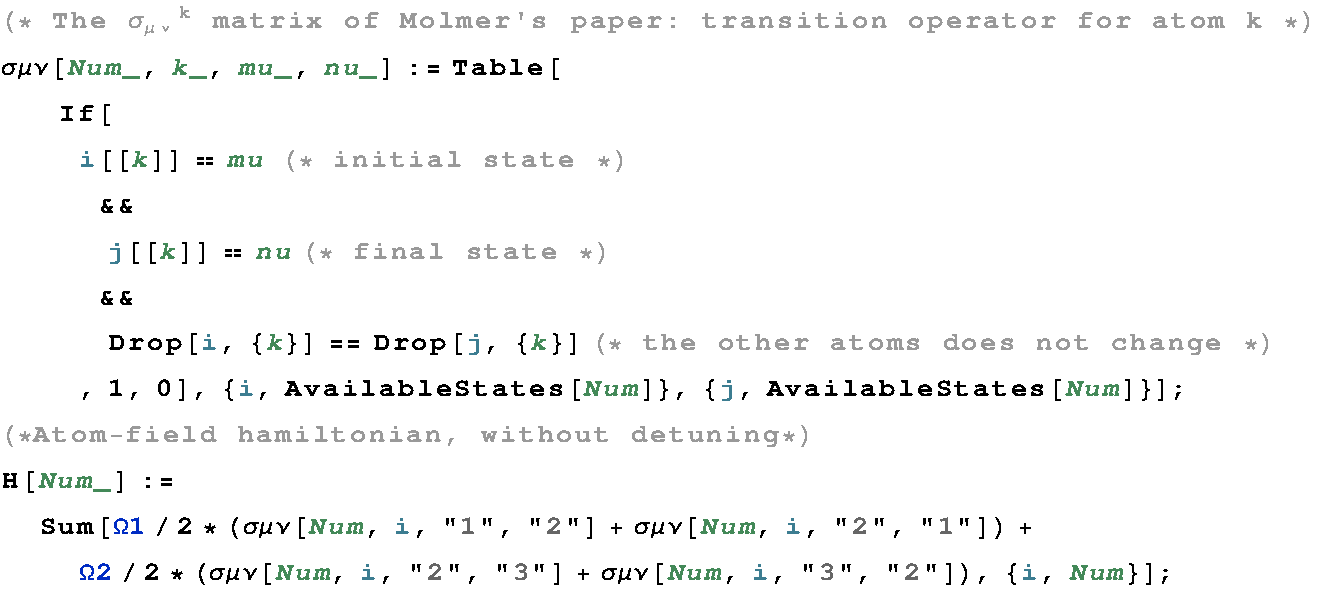
\includegraphics[width=0.8\textwidth]{MathematicaSampleCode.pdf}
  \caption{\label{Mathematica-code}\mat code to implement $\sum_j \mc{V}_{\mathrm{af}}^j$ using \emph{functionnal} programming}
\end{figure}

\begin{wrapfigure}{r}{0.45\textwidth}
  \vspace{-10pt}
  \centering
  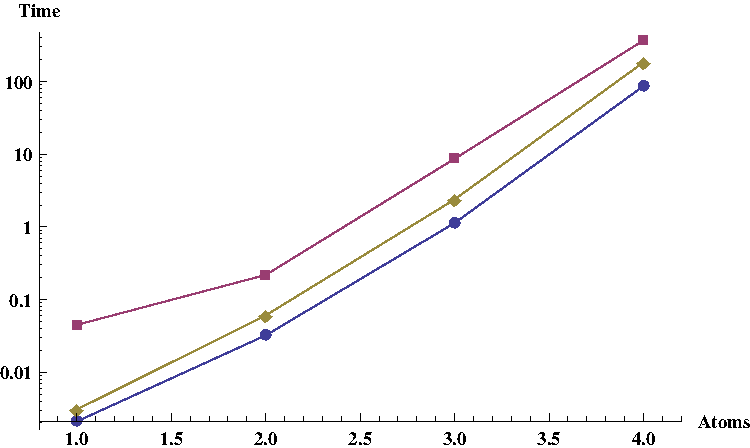
\includegraphics[width=0.45\textwidth]{benchmark.pdf}
  \caption{\label{benchmark-plot}Master equations computation time}
  \vspace{-20pt}
\end{wrapfigure}


\par This example shows an optimisation of the previous code. Such a work is not useless because the number of available states varies exponentially with the number of atoms. The \Cref{benchmark} and \Cref{benchmark-plot} give the time needed to find the master equation. This shows that my code\footnote{The reader should be aware that Calum's code does not give the same master equations as the other ones.} is the fastest, however the master equation has to be found only once. Then the interesting task is to solve it for different initial conditions and laser excitation. The master equations can be written into text files for large number of atoms. Indeed the \Cref{benchmark-plot} shows that the computation grows as the size of the density matrix, it means exponential with the number of atoms. This fast growth is linked to the states in superposition. It is hard to simulate the behaviour of quantum system using a classical computer.

\begin{table}[h]
  \centering
  \begin{tabular}{||l||c c c c||}
    \hline
    Number of atom & 1 & 2 & 3 & 4\\
    \hline \hline
    Calum's code & 3.1ms & 60.5ms & 2.39s & 3min4s\\
    Ilya's code & 44.8ms & 218ms & 8.65s & 6min8s \\
    My code & 2.1ms & 32.1ms & 1.13s & 1min27s \\
    \hline
  \end{tabular}
  \caption{\label{benchmark}Benchmark of several codes to find the master equation}
\end{table}

\section{Modelling experiments}

\par The implementation of master equation had been mainly motivated by two reasons. The first one was to try to validate a theoretical proposal of my supervisor about a means to derministically excite one single atom using a chirped laser pulse. He tried to validate his idea by numerical simulations, but at that time the decay was not implemented properly. This new implementation will then be useful to revalidate this proposal.

\par On the other hand an accurate theoretical model could be useful to predict \emph{a priori} or analyse \emph{a posteriori} the experiments. 

\subsection{STIRAP}

\begin{wrapfigure}{r}{0.5\textwidth}
  \vspace{-10pt}
  \centering
  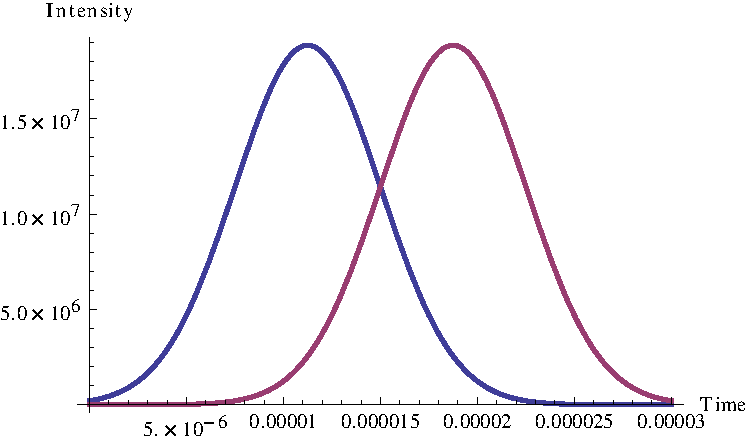
\includegraphics[width=0.5\textwidth]{STIRAP-seq.pdf}
  \caption{\label{STIRAP-seq}STIRAP laser pulse sequence\\$\Om_{ge}$ in red and $\Om_{er}$ in blue}
  \vspace{-10pt}
\end{wrapfigure}

\par The STImulated Raman Adiabatic Passage is method used to populate the Rydberg state despite the $\sqrt{N}$ dependency of the collective Rabi frequency. It consist in a two laser pulses sequence sent in a counterintuitive order. The first one $\Om_{er}$ is tunned to the transition from \ee to \rr, and the second one $\Om_{ge}$ to the transition from \ff to \ee. The \Cref{STIRAP-seq} shows the pulse sequence used to first reproduce Mølmer's results. During this sequence, a quantity defined by the following expression and called the \emph{mixing angle} $\Theta$ is swept from $0$ to $\pi/2$: \[ \tan \Theta \defi \frac{\Om_{ge}(t)}{\Om_{er}(t)} \]

\par This mixing angle could be used to express the eigenstates of the atom-field interaction hamiltonian $\mc{V}_{af}$ in the case of resonant coupling. For one atom, \cite{Berg} gives the following expressions: 

\begin{align*}
\ket{a^+} &= \sin \Th \sin \Phi \ff + \cos \Phi \ee + \cos \Th \sin \Phi \rr \\
\ket{a^0} &= \cos \Th \ff - \sin \Th \rr \\
\ket{a^-} &= \sin \Th \cos \Phi \ff - \sin \Phi \ee + \cos \Th \cos \Phi \rr
\end{align*}

\par In these expression $\Phi$ is also a function of Rabi frequencies, but it not relevant. The important information is that while the mixing angle $\Th$ runs from $0$ to $\pi/2$ allows the state \ee is never populated as it is described in the \Cref{sweeping}. The initial state is $\ff = \ket{a^0}$, and during the mixing the atom stands in state $\ket{a^0}$ because it an eigenstate of the hamiltonian.

\begin{table}[h]
  \centering
  \begin{tabular}{||c||c c||}
    \hline
    $\Th$ & $0$ & $\pi/2$\\
    \hline \hline
    $\ket{a^+}$ & $\cos \Phi \ee + \cos \Th \sin \Phi \rr$ & $\sin \Phi \ff + \cos \Phi \ee$\\
    $\ket{a^0}$ & $\ff$ & $-\rr$\\
    $\ket{a^-}$ & $- \sin \Phi \ee + \cos \Phi \rr$ & $\cos \Phi \ff - \sin \Phi \ee$\\
    \hline
  \end{tabular}
  \caption{\label{sweeping} Values taken by the eigenstates at the initial and last position \\ of the mixing angle $\Th$}
\end{table}

\par It has been shown that this sequence, based on gaussian pulses delayed by their width, has the lowest losses from non-adiabatic coupling to the $\ket{a^+}$ or $\ket{a^-}$ \cite{Berg}. This sequence can then be used in addition to the master equation to numerically simulate the STIRAP. This has been done in \cite{Molmer} and reproduced by my program\footnote{A complete version of the code is availaible at this address: \url{https://github.com/thriller91/Quantum-gates\_Rydberg-atoms}}. The \Cref{STIRAP-exp} shows a STIRAP sequence applied to a 3~atoms gaz with resonant lasers ($\delta_1 = \delta_2 = 0$), a laser intensity of $\Om_0 = \SI{2 \pi 3 \cdot 10^6}{rad/s}$, a dipole-dipole interaction strengh of $\Delta = \SI{10^{10}}{rad/s}$, spontanous decays of $\Ga_{ge} = \SI{38}{MHz}$ and $\Ga_{re} = \SI{1}{kHz}$, and finally, the time duration of the pulses sequence is $\Ga_{ge} = \SI{30}{\micro s}$.

\begin{figure}[h]
  \centering
  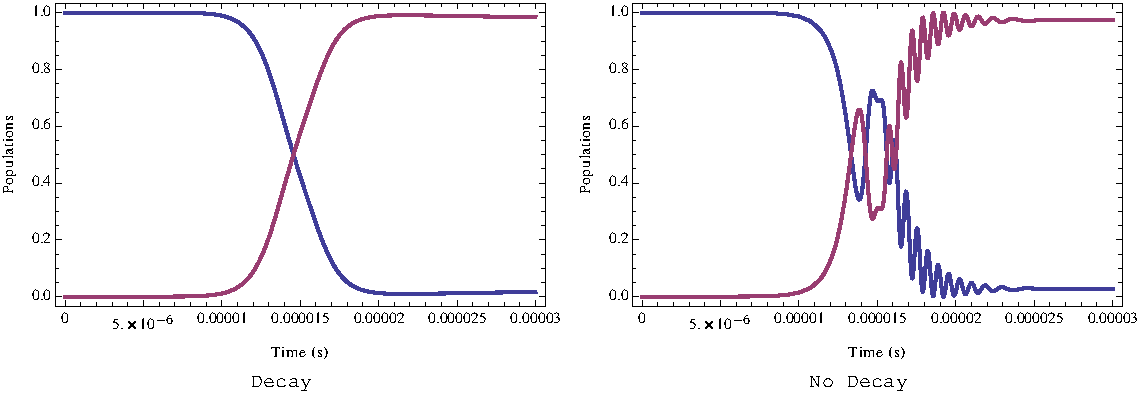
\includegraphics[width=0.9\textwidth]{STIRAP-exp.pdf}
  \caption{\label{STIRAP-exp}Probability not to have any atom in Rydberg state (in blue) or only one single (in red) after a STIRAP sequence,\\ with (on left) or without (on right) taking into account spontaneous decay}
\end{figure}

\par In this figure, one can notice the fast oscillations when there is no decay in the equations. It due to a non desirable population of state \ee, it naturally happens with large number of atoms because of the unstability of the system. But if this state \ee decays to \ff, this effect is no more visible, at least for $N=3$ atoms. Moreover, the final probability to excite one single Rydberg atom is smaller than in the case without decay, the authors of \cite{Molmer} explain it means adiabaticity condition is then no more valid. The \Cref{STIRAP-state-e} and \Cref{STIRAP-adiab} given in \Cref{annexe} highlight the population of state \ee in the case where it does not decay to \ff and a violation of the adiabaticity by reducing of the time duration of the pulses sequence.

\subsection{CHIRP}

\par In \cite{Ilya} our team has emitted a theoretical proposal about another deterministic way to excite one single atom. It is based on a laser pulse in which the frequency is swept, this is called a chirped pulse (CHIRP). Like the STIRAP method, this one can be used to make a rapid adiabatic passage and then overpass the $\sqrt{N}$ dependance. The main difference is that CHRIP employes only one laser instead of two for STIRAP. It has been shown that these two techniques are equivalent in principle \cite{Berg}.

\par In his article, my tutor shows numerical simulations for a two atoms system. However, these simulations were based on the quasi-molecular model which is briefly explained in \Cref{qm-model}. There was two interesting informations in these simulations. Unfortunately, I have not been able to reproduce them with my program based on the \Cref{master-eq}.

\par Firstly, he has shown that CHRIP could be used to make a deterministic excitation of one single atom if one uses large detuning from the intermediate state \ee. I have tried with 3 atoms but I did not managed to excite efficiently one single atom. Secondly, he has noticed a chaotic behaviour of the population with respect to the detuning from the intermediate state. This behaviour does not appear even if I chose zero decays. It is a bit hard to dive into the \mat code of my supervisor based on the quasi-molecular model. I hope he will easily dive into mine and find our divergences.

\section{Rydberg blockade criterion}

\par The key point is the Rydberg blockade. The team of Mark Saffman managed to get it \cite{CNOT}, as well as some teams form other countries. The \Cref{igor-ryd} at the end of this section shows a first proof of Rydberg blockade in our experiment. The specificity of our team is the electron counter used for the measurement. The atoms are between two metallic plates. An electric field is applied to gradually ionise the eventual Rydberg atoms of each level. Then the electrons are collected by the counter, which can count at maximum 5 electrons. Each experiment is repeated 5000 times to improve the signal-to-noise ratio.

\par At the end of my internship, my supervisor made a 3 weeks trip in U.K. to visit the partner team of Silvia Bergamini at the Open University. While he was absent I worked with Igor on theoretical model close to our current experiments. He was working on a theoretical model to release a clear criterion to claim whether there is Rydberg blockade in our experiments.

\subsection{The quasi-molecular model \label{qm-model}}

\par Here we consider a two-level system with a ground state \ee and Rydberg state \rr the former ground state \ff is never populated and $\Ga_{eg}=0$. Igor used to model a two atoms system like a quasi-molecule. They could be in 4 different states: the ground state $\ket{ee}$, two symmetrical states $1/\sqrt{2} (\ket{re} +\ket{er})$ and $1/\sqrt{2} (\ket{re} -\ket{er})$ and the excited state $\ket{rr}$. Then he writes down the optical Bloch equations by hands and he adds decays and lasers linewidth. Finally, he reduces the number of equations from 16 to 7.

\par On the other hand, he writes the following expression, where $\Om$ is the Rabi frequency of the laser, $\delta$ the detuning to the transition \ee to \rr, and $\Ga$ the decay rate of \rr to \ee:
\begin{equation}
 \mc{P} = \frac{\Om^2/2}{2\delta^2 + \Ga^2/2 + \Om^2} \label{rabi-eq}
\end{equation}
The probability to excite one atom. Then if there are two or more atoms, statistics are described by a binomial distribution. For two atoms, the probability to excite the two atoms is $p_2 = \pp^2$, the probability to excite one of the two atoms is one half\footnote{There are two equiprobable ways to excite one atom.} of $2 p_1 = 2 \pp (1-\pp)$ and finally the probability not to excite any atom is $p_0 = (1-\pp)^2$. Then is comes that a quantity called $\theta$ by Igor have to be equal to zero: \[ \theta \defi 1 - \frac{p_2}{(p_1 + p_2)^2} \]

\par This quantity is modified when there is Rydberg blockade, because $p_2$ changes. I have used my program based on Mølmer's article to see how the spectra must evolve. To do so and obtain \Cref{theta-plots} I have chosen constant Rabi frequency $\Om = \SI{1}{Hz}$, an arbitrary decay $\Ga = \SI{1}{Hz}$ and the detuning was swept to draw the spectrum. Under theses conditions, the system of two atom should oscillate at the Rabi frequency, the oscillations damped to stationary value given by \Cref{rabi-eq}. The time of the experiment was chosen longer enough to get the stationary value, $\tau = \SI{4}{s}$ had been a good choice.


\begin{figure}[h]
  \centering
  \begin{subfigure}[b]{0.5\textwidth}
  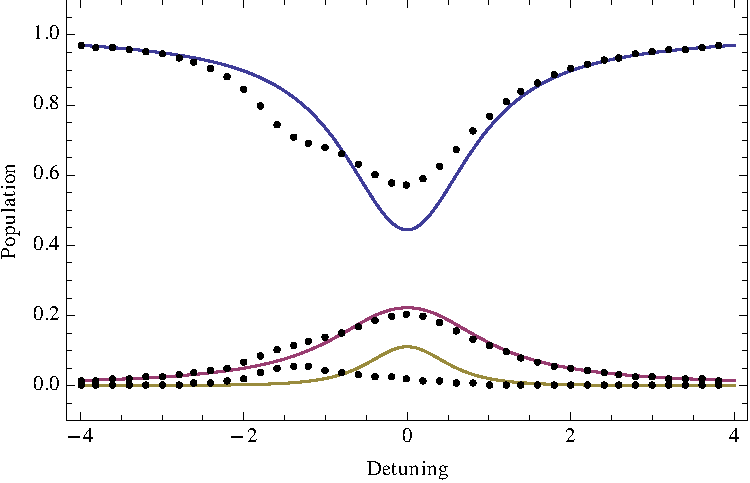
\includegraphics[width=0.9\textwidth]{blockade-sp.pdf}
  \caption{\label{theta-sp}Spectrum done with a dipole-dipole interaction strength $\Delta = \SI{3}{Hz}$ \\ Solid lines: plot of \cref{rabi-eq}; dots: simulations \\ blue: $p_0$; red: $p_1$; yellow: $p_2$}
  \end{subfigure}
  ~
  \begin{subfigure}[b]{0.5\textwidth}
  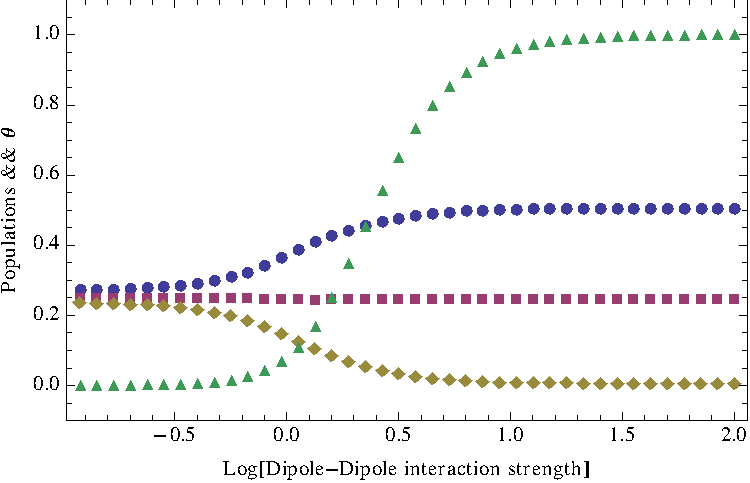
\includegraphics[width=0.9\textwidth]{blockade-semilog.pdf}
  \caption{\label{theta-log}Semi-log plot of the populations and $\theta$ parameter on the range $\Delta =$ [0.1; 100] \\ blue circle: $p_0$; red square: $p_1$; yellow diamond: $p_2$; green triangle: $\theta$}
  \end{subfigure}

  \caption{\label{theta-plots} Spectrum and plots that shows Rydberg blockade in theory}
\end{figure}

\par Such evolutions are trivial: if $\Delta$ increase smoothly, $p_2$ should decrease smoothly then $\theta$ has to go from $0$ to $1$ smoothly. However the behaviour of the spectrum for intermediate dipole-dipole strength is not obvious: it creates a second resonance that is shifted to the red. In practice Rydberg blockade is easy to handle because the atoms are not sensitive to its variations when it is stronger enough \cite{Saff-rev}.

\subsection{Pursuit of Rydberg blockade in experimental data}

\par The experimental setup allows us to measure the signals of one, two, three, four and five atoms. These signals are writen $S_k$. The total signal $S$ is given by $S = p N_0 T = \sum_{N=1}^{N_0} N P_N$, where $N_0$ is the total number of atoms in the interaction volume, $p$ is the probability to excite one atom, $P_N$ is the probability to detect $N$ atoms and $T$ is the yield of the detector. The probability $P_N$ to detect $N$ atoms follows a binomial low: \[ P_N = (pT)^N (1-pT)^{(N_0-N)} \frac{N_0!}{N! (N_0-N)!} \]

\par From two previous formulas, one can compute the multi-atom signal\footnote{The detector multiplies the signal by $N$ when it detects $N$ atoms.}: \[ S_N = N \left(\frac{S_0}{N_0}\right)^N \left(1-\frac{S_0}{N_0}\right)^{(N_0-N)} \frac{N_0!}{N! (N_0-N)!} \]

\par When the probability $p \ll 1$, this distribution could be approximated to a Poisson distribution. Then the multi-atom signal is independent of $N_0$, the number of atoms in the interaction volume: \[ S_N = N \frac{S^N}{N!} e^{-S} \]

\par Igor gave me two experiment data files to analyse. The first was done under Forster resonant and the second was off-resonant. An additional electric field is tune Stark effet across the middle between two Rydberg states energies which is called the Forster resonance. At this point, two Rydberg atoms are created and Rydberg blockade is enhanced. The \Cref{forster} shows that when the electric field is Forster off-resonant, the $\theta$ parameter is flat and little close to the microwave resonance\footnote{The signal out of resonance is meaning less, because too noisy.}. The difference between between the plots could be small, but it exists and it is consistent with the theory. These graphs have been made considering $N_0 = 5$ and using a binomial distribution\footnote{The code and the experimental data files used can also be found on \url{https://github.com/thriller91/Quantum-gates_Rydberg-atoms}}.

\begin{figure}[h]
  \centering
  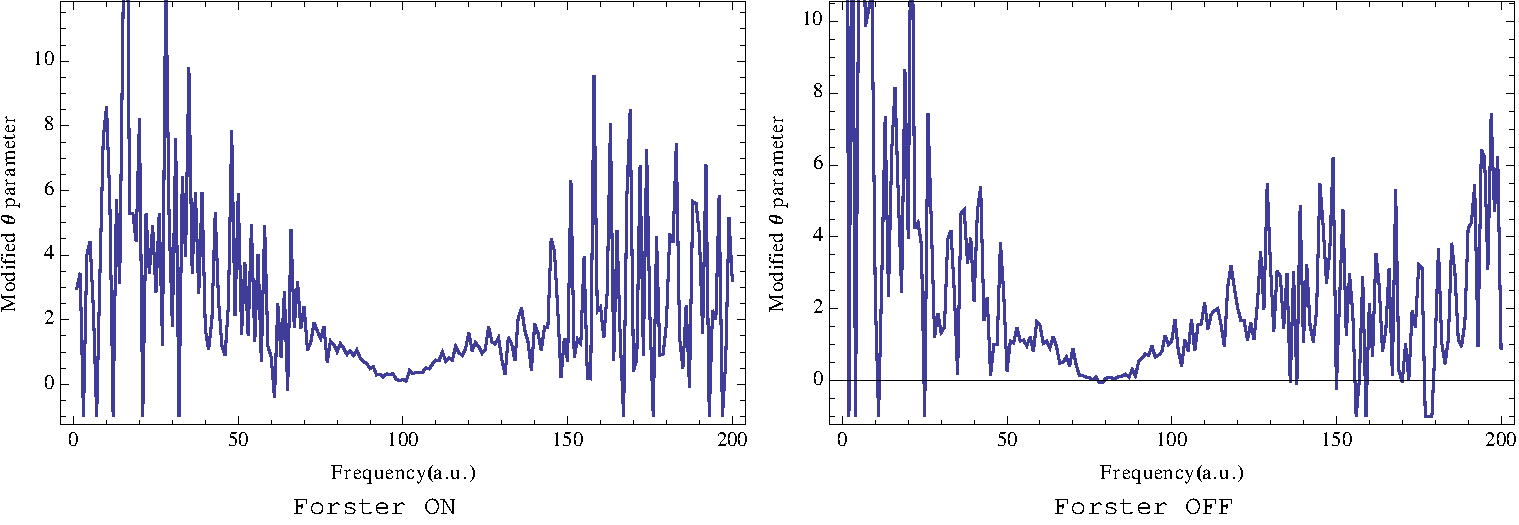
\includegraphics[width=0.8\textwidth]{forster.pdf}
  \caption{\label{forster} Rydberg blockade enhanced by Forster resonance \\ Plot of the $\theta$ parameter, it should be equal to zero\\ in absence of Rydberg blockade}
\end{figure}

\par This work has been a preliminary one, Igor was satisfied in spite of the non-spectacular proof of Rydberg blockade. He had tried him self to directly plot experimental data under some special scale, and he has found the \Cref{igor-ryd}. This figure shows that is multi-atom excitations higher than 2 atoms are less frequent under Forster resonance. This proof is also not really obvious but anyway Igor was enthusiastic because this experiment was done with Rydberg state with principal quantum number $n \sim 37$, and they have planned to move to high levels $n \sim 80$ for the next experiments.

\begin{figure}[h]
  \centering
  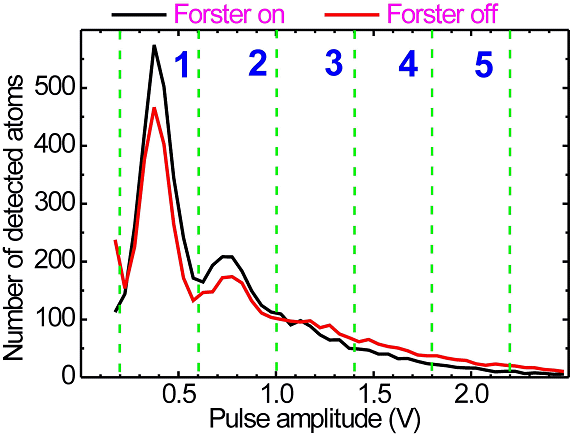
\includegraphics[width=0.5\textwidth]{igor-ryd.png}
  \caption{\label{igor-ryd} Pure experimental data showing a weak Rydberg blockade\\ The number at the top shows the number of simultaneous\\ Rydberg atom detected in the interaction volume}
\end{figure}

\chapter{Automation of atom excitation}

\par During my internship several experimental tasks have been proposed to me by my supervisor. These tasks have been done simultaneously with my theoretical jobs. As a typical intern, they were mainly about programming. Furthermore working in a Quantum Optics team does not require skills in Optics as expected but in Electronics and IT, especially in Russia. The optical devices are used to shine the Rb atoms and make experiments. But these devices need electronic support like stabilised power supply, noise eater or synchronisation.

\par A research work is supposed to be at the state of the art. It then needs some very specific materials which are either very expensive or time consuming because they are home-made. A team has to optimise its efficiency with a finite budget. Russian physicists (except academicians) are not well paid. That is why is might be cheaper to use the laboratory workforce. The strategy of building everything in the laboratory has two main issues. Firstly, researchers are wasting time when they are building material that is already commercially available. Secondly, non-specialists can hardly get to the same level as industrial (time delay, quality, guaranty, etc.). That is why our team usually spend its money from grants to buy some equipments from abroad in spite of the huge customs fees.

\par Then I have learnt how to find second-hand capacitors on old electronic cards to improve and make our own devices. That kind of electronics and programing jobs are essential to modernise the experimental setup.

\section{Control of the time sequence of the lasers}

\par After all the experiments I used to treat the acquired data with \emph{Origin} and the next day we used to go Igor's office to discuss the results. It was interesting to see how he asked the good questions to clarify his ideas on the records. He employed the word ``pedestal'' where I used ``noise'', I mean he analysed data very accurately. One question has been asked all the meetings: ``What was the time sequence?'' This question was sometimes embarrassing for the team, because all the members were not sure of their pulse duration and intensity. A real control of the time sequence of the lasers is mandatory to give us the hope to one day see actual quantum algorithms running.

\subsection{Timers}

\par A \emph{\textbf{ADLink PCI-8854}} card which contains 12 timers/counters was installed the main computer of the experimental room. This card was unused for some years and the adaptation circuit made by Vassili. My goal was to get as many output delayed rectangular pulses as I can, moreover these pulses have to be controled by the global \emph{LabVIEW} program that manage all the experiment (data acquisition, live visualisation of an histogram of multi-atom signals, data recording, etc.). These pulses will be used to control acousto-optical-modulator and create laser pulses for the experiments. Previously all the pulses were generated separately by each laser user, then delayed was synchronised on a oscilloscope. This system will allow a centralised management of the delays and durations of each pulses.

\par The former implementation by Vassili had not the same purpose, but anyway it was obsolete and I have restarted from scratch with the latest \emph{LabVIEW} driver. The idea is to use one time to gate another one in order to delay it. Then 2 timers are required to make 1 delayed pulse. The \Cref{timers} shows how to gate two timers to get a delayed pulse. However the 2 last timers cannot be used because they are mechanically cascaded and 1 more timer was broken. I finally managed to get 4 delayed pulses and 1 non-delayed pulse. 

\begin{figure}[h]
  \centering
  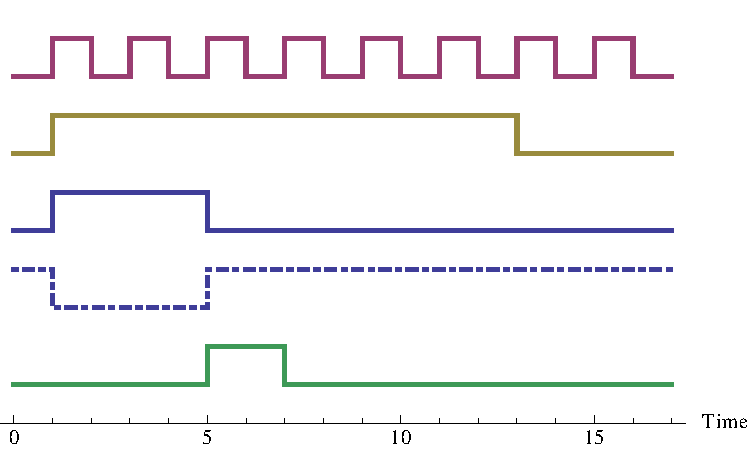
\includegraphics[width=0.5\textwidth]{timers.pdf}
  \caption{\label{timers}How to configure counters to get delayed pulses\\
(red) \texttt{global clock} 8MHz \\
(yellow) \texttt{timer 11}: periodic mode, counts: 6; \emph{Periodicity of the pulse}\\
(blue) \texttt{timer 1}: gated on 11, counts: 2; \emph{this is the delay}\\
(blue dotted) \texttt{timer 1}: \emph{the signal is actually inverted} \\
(green) \texttt{timer 2}: gated on 2, counts: 1, \emph{here is the delayed pulse}}
\end{figure}

\par And once we get delayed pulses we have to send them to the experimental setup. Vassili helped me find the right transistors to amplify these signals: we found the transistors in an old TV set, and the 12V power supply was a mobile phone adapter. He asked me to put opto-couplers to make an electric separation between the computer and the experimental setup where high voltages are applied for ionisation. The bottom line is that it worked. We tried it with Vassili's part of the experiment and also Denis' one.

\subsection{Arbitrary waveform generator}

\par An electric field is applied to the atoms through two parallel metallic plates. This field was previously applied with old electronic devices that were put together to draw a small rectangular pulse before the ionisation ramp. Igor noticed a fast oscillation in the experimental records. He guessed the origin of these oscillations was in the electric field applied, and it was the case. Then he suggested me to use the \emph{\textbf{PicoTest  G5100A Waveform Generator}} to generate an externally triggered signal of two rectangular pulses with sharp edges.

\begin{wrapfigure}{r}{0.5\textwidth}
  \vspace{-10pt}
  \centering
  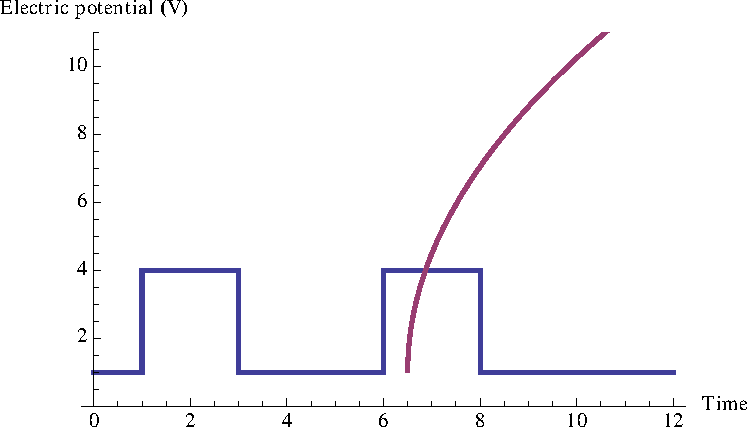
\includegraphics[width=0.5\textwidth]{overlap.pdf}
  \caption{\label{overlap}Overlapping of the electric pulses}
  \vspace{-20pt}
\end{wrapfigure}

\par The second pulse overlaps the ionisation ramp as shown in \Cref{overlap}. But this does not matter because only the maximum of the two signals is applied due to the diodes inside the experimental setup (\Cref{dubdub}). The goal of this second pulse is to avoid dirty oscillations at the beginning of the ionisation ramp, indeed the \emph{PicoTest} generator is supposed to have sharper edges. The effect of the permanent electric field and the delay between the two pulses will be studied in next experiments.

\vspace{2em}

\begin{figure}[h]
  \centering
  \scalebox{0.7}[0.7]{
		\begin{circuitikz} 
		\begin{scope}[scale=1]
		\filldraw [fill=white,draw=black] (-0.5,0) circle (0.5cm) node {$\Om_{pls}$};
		\draw (0,0) -- (1,0);
		\draw (1,0) -- (1,1.5);
		\draw (3,0) to[D] (1,0);
		\draw (3,1.5) to [C] (1,1.5);
		\draw (3,1.5) -- (3,0);
		\draw (3,0) -- (7,0);
		\draw (4,0) to [R] (4,-2);
		\begin{scope}[scale=0.4]
			\draw (9.25,-5) -- (10.75,-5);
			\foreach \x in {9.25,9.5,9.75,10,10.25,10.5,10.75}
				{
				\draw (\x,-5)--++(-0.5,-0.5);
				}
		\end{scope}
		\draw (6,0) to [C] (6,-2);
		\begin{scope}[scale=0.4]
			\draw (14.25,-5) -- (15.75,-5);
			\foreach \x in {14.25,14.5,14.75,15,15.25,15.5,15.75}
				{
				\draw (\x,-5)--++(-0.5,-0.5);
				}
		\end{scope}
		\draw (7,0) -- (7,1.5);
		\draw (7,0) to[D] (9,0);
		\draw (7,1.5) to [C] (9,1.5);
		\draw (9,1.5) -- (9,0);
		\draw (9,0) -- (10,0);
               \filldraw [fill=white,draw=black] (10,0) circle (0.5cm) node {$\Om_{ioni}$};
		\node at (-0.5,-1.5) {pulse generator};
		\node at (10,-1.5) {ionisation signal};
		\end{scope}
		\end{circuitikz}
  }
  \caption{\label{dubdub} Schematic diagram of the experimental setup\\ The diodes help to take the maximum of both generator\\ (at first $\Om_{pls}$ and then $\Om_{ioni}$) \\ The ionisation plates are represented like a capacitor\\ in the middle, next to the parasitic capacitance}
\end{figure}

\section{Renew of the experiment}

\par There were two places where I was working at the Institute of Semiconductor Physics: the office of my supervisor at the first floor and the experimental room at the ground floor. The first day I came, I have seen the experimental setup and I was really amazed. It was a mixture of Soviet time stuff and modern equipments which are not very surprising because they are miniaturised and simplified. Some interesting Soviet devices were still working, like a spectrum analyser up to a few GHz.

\par A new Russian electronic industry has to emerge, because since the collapse of the Soviet Union, Russian laboratories are dependant on foreign importations. This situation creates a high latency in Research, due to the shipping and customs checking delays. Moreover, researchers have to find the best material at the cheapest price with respect to customs fees. That push them to do the most they can in their own workshop, and then to do things they are no supposed to do and spend time on tasks they are not specialised in.

\par Each permanent member of the team was responsible of his laser and his parts of the experiment in addition to some global parts. They were handling their own lab journal in which they used to put the important modifications they brought to their part of the experimental setup. But to me this was like a famous recipe from which the chiefs want to jealously keep the secret. The PhD student could replace my supervisor, but I wondered what might happen if another permanent member have to be absent for a while. The experimental setup needs to be simplified to prevent a big failure, save time and get better results.

\subsection{Microwave spectroscopy}

\par The first time I visited the experimental setup, my supervisor explained me what they were working on using a poster. When we were leaving the room, in the corner was half a dozen of old Soviet devices, staked on wheels. I was hardly taller than the whole. My tutor told me that this set of old devices is used to generate microwave and it has to be replaced by a new compact solution, namely the \emph{\textbf{Agilent E8257D PSG Analog Signal Generator}}.

\par A microwave generator is required to make microwave spectroscopy of the Rydberg states. Indeed, the transition between different Rydberg levels is in this range of energy. Unlike their laser spectroscopy setup, this one was able to give an absolute frequency\footnote{I was in charge of experimental data treatment. In order to get the frequency range of the spectra, I knew that there were two known resonances distant from $\SI{92.5}{MHz}$ and I used to fit the range on these resonances when they were both visible. I used to use a mean range otherwise.}. It was still work and used during my internship. It was composed of power supplies, generator, amplifiers and feedback analyser.

\par All these devices could be replaced by the \emph{Agilent} microwave generator. But unfortunately we had not been able to try it before the end of my internship because we received the output cable that Denis had ordered in May two weeks before I left, in July. I made a program under \emph{LabVIEW} and included it into the global program of the experiment. The program has been tried properly without enabling the output\footnote{Actually my supervisor was worried about using it without the output cable or another $50\Om$ charge.}.

\par The generator is connected to the remote computer with a Ethernet cable. I have chosen not to use Serial connection because it is slower, or GPIB because it has limited length and it is harder to find. It was also possible to connect the generator to the router, then it would have been possible to use it with all the computer connected to the local network. Nonetheless, for the sake of security, we have decided to make a special connection to the main computer of the experimental room.

\par The computerisation and automation of the experiment is compulsory to obtain better results. Generally speaking and particularly in this setup, which is a mixture of modern and Soviet time devices, the sophistication of the experiment slows down with the increasing of its complexity. The new microwave generator will simplify the setup and must lead to better experimental results.

\subsection{New vacuum system and outlook}

\par Some few weeks after my arrival, we received metallic pieces to make the new vacuum system. All the team was busy with experiments till the summer. While my supervisor was absent I also worked worked with Denis on the vacuum system.

\par It has a better pump than the previous one and also larger windows. This could be useful because the larger are the windows, the more the laser beams could be focused. For now we are using \emph{magneto-optical trap}. A focused gaussian laser beam can be used to make a \emph{dipole trap}, which could be used to draw new trapping geometries like arrays that are interesting for quantum information. 

\par But this part of the experiment, which was new and independent from the remaining was not a priority. When they received the parts, they sent some to the workshop of the laboratory to solder them using non-magnetic process. Then we have tried the vacuum pump: \emph{\textbf{Pfeiffer-Vacuum HiCube Eco 80}} and its gauge for vacuum measurement. This pump has two stage, the first one is a diaphragm pump. It consist of a chamber in which takes place a motor that push a diaphragm to have a linear movement like a piston. Two valves make the connexion between the vacuum chamber and pumping chamber, and between the pumping chamber and the atmosphere. This pump can reach an ultimate pressure of about $\SI{70}{mbar}$ \cite{Pfeiffer}. The second stage is made of a turbo-molecular pump. Its principle is the same of a simple fan, a turbine rotates at a very high speed (typically $90000$ tr/min), its blades give impulses to the gas molecules to push them to the outlet.

\par At first we faced a problem, when we had launched the system, the pressure reached quickly a local minimum at about $\SI{10^{-3}}{mbar}$ prior to slowly increase. The pump has a timeout of $\SI{8}{min}$, after this delay, it stops if it has not reached its final rotation speed setpoint. We solved this issue by tightening again the nuts. To me, a leak cannot explain this issue, because there might not be any \emph{local} minimum if there were a leak. Anyway there no problem anymore, as a matter of fact we easily reached a pressure of $\SI{10^{-8}}{mbar}$.


\addchap{Conclusion}

\begin{quotation}
\emph{Physics is really nothing more than a search for ultimate simplicity, but so far all we have is a kind of elegant messiness.} \\
--- Bill Bryson, \emph{A Short History of Nearly Everything}
\end{quotation}

\nocite{*}
\bibliographystyle{alpha}
\bibliography{optiquequantique}

\appendix

\chapter{\label{annexe}Additional figures}


\begin{figure}[h]
  \centering
  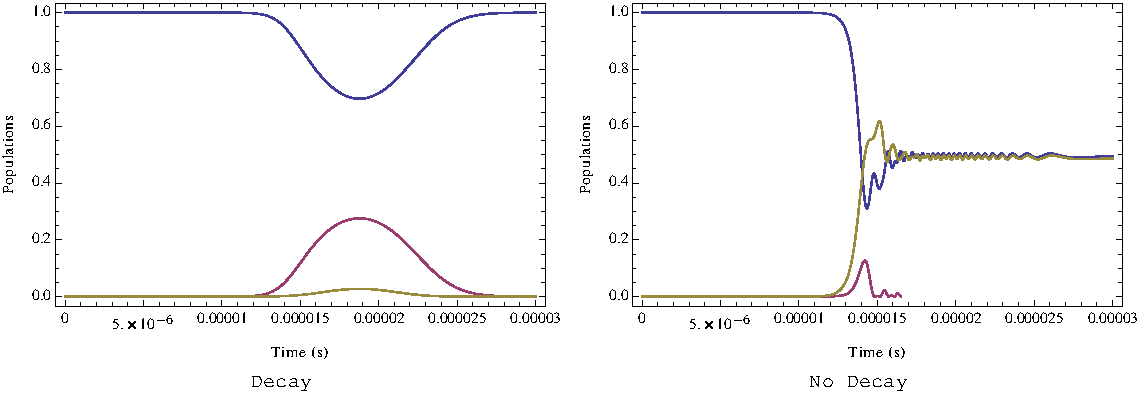
\includegraphics[width=1\textwidth]{STIRAP-state-e.pdf}
  \caption{\label{STIRAP-state-e} Graph of the \ee state population for STIRAP experiment with 3 atoms \\
(blue) no atoms in state \ee; (red) one atom in \ee; (yellow) two atoms in \ee \\
We can notice that in presence of decay from \ee to \ff, the population of \ee is low especially at the end of the experiment}
\end{figure}

\begin{figure}[h]
  \centering
  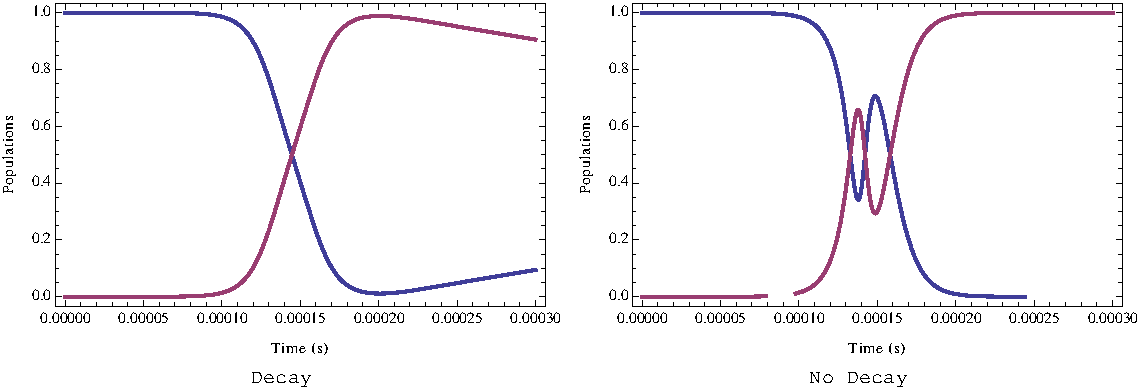
\includegraphics[width=1\textwidth]{STIRAP-adiab.pdf}
  \caption{\label{STIRAP-adiab} Probability to excite one single Rydberg atom (blue) or no Rydberg atom at all (blue) during a \emph{shortened} STIRAP experiment; this shows a violation of adiabaticity}
\end{figure}

\end{document}
